\documentclass[sans, mathsans, russian]{beamer}

% http://faq.ktug.org/wiki/uploads/MathFonts.pdf
\usepackage{pxfonts} % pxfonts or palatino or mathpazo packages
\usepackage{eulervm}

\usepackage{mystyleslides}
\usepackage{cohmystyle}
\usepackage{changepage}

% https://tex.stackexchange.com/questions/1656/footnote-counter-would-like-to-restart-from-1-each-page
% https://stackoverflow.com/questions/3701605/how-to-restart-footnote-numbering-every-page

% \usepackage[perpage]{footmisc}

% \usepackage{perpage}
% \MakePerPage{footnote}

%% \usepackage{eulervm}
%% \usepackage{fourier}

\graphicspath{ {images/} }

\usetheme{Warsaw} % Warsaw Copenhagen Madrid CambridgeUs Darmstadt Frankfurt Singapore
\setbeamertemplate{headline}{}

\definecolor{beamer@blendedblue}{RGB}{8, 37, 103}
%% 13, 74, 76 -- pre-defence
%% 0, 65, 106 *
%% 0, 51, 102
%% 8, 69, 126
%% 0, 49, 83

%% 17, 96, 98
%% 1, 58, 51

\definecolor{my-red}{RGB}{176, 0, 0}
\definecolor{my-blue}{RGB}{0, 0, 153}
\definecolor{my-teal}{RGB}{0, 153, 153}
\definecolor{my-green}{RGB}{0, 153, 0}
\definecolor{my-violet}{RGB}{75, 0, 130}
\definecolor{my-pink}{RGB}{253, 123, 124}
%{90, 45, 102} % violet
%{145, 30, 66} % light cherry
%{146, 43, 62} % cherry

%\usecolortheme{default}
%\usecolortheme{sidebartab}
%\usefonttheme{default}

% Inserting frame numbers in footline
% http://tex.stackexchange.com/questions/191198/customization-of-the-copenhagen-theme
\makeatletter
  \iffalse
  \pgfdeclarehorizontalshading[frametitle.bg,frametitle right.bg]{beamer@frametitleshade}{\paperheight}{%
    color(0pt)=(myblue2);
    color(\paperwidth)=(white)}
  \fi

  \defbeamertemplate*{footline}{mysplit theme}
  {%
    \leavevmode%
    \hbox{\begin{beamercolorbox}[wd=.5\paperwidth,ht=2.5ex,dp=1.125ex,leftskip=.3cm plus1fill,rightskip=.3cm]{author in head/foot}%
      \usebeamerfont{author in head/foot}\insertshortauthor
    \end{beamercolorbox}%
    \begin{beamercolorbox}[wd=.5\paperwidth,ht=2.5ex,dp=1.125ex,leftskip=.3cm,rightskip=.3cm plus1fil]{title in head/foot}%
      \usebeamerfont{title in head/foot}\insertshorttitle\hfill
      \insertframenumber\ / \inserttotalframenumber\hspace*{0.5em}
    \end{beamercolorbox}}%
    \vskip0pt%
  }
\makeatother


% https://tex.stackexchange.com/questions/170222/change-the-numbering-in-beamers-table-of-content
%\makeatletter
%\patchcmd{\beamer@sectionintoc}
%  {\ifnum\beamer@tempcount>0}
%  {\ifnum\beamer@tempcount>-1}
%  {}
%  {}
%\beamer@tocsectionnumber=-1
%\makeatother


%\setbeamertemplate{footline}[frame number] % page numbering outside Navigation Bar
\setbeamertemplate{navigation symbols}{} % switch off navigation bar
%\setbeamertemplate{caption}[numbered]

\setbeamertemplate{itemize item}[ball] % Загадка, но без этого у itemize не будет кружочков % itemize items
\setbeamertemplate{itemize subitem}[triangle]
\newcommand{\labelitemi}{\usebeamertemplate{itemize item}{}} % Загадка, но без этого у itemize не будет кружочков
\newcommand{\labelitemii}{\usebeamertemplate{itemize subitem}{}} % https://tex.stackexchange.com/questions/12735/can-one-replace-bullet-points-with-graphics


%\AtBeginSection[]
%{
%  \begin{frame}
%    \frametitle{Содержание}
%    \tableofcontents[currentsection]
%  \end{frame}
%}


\title[Внутритекстовая когерентность]
{
  Внутритекстовая когерентность\\
  как мера интерпретируемости\\
  тематических моделей текстовых коллекций\\
}
\subtitle{}

\author[Василий Алексеев]{
  Василий Алексеев
}

\institute[]
{
  \footnotesize
  % MIPT
  % 
\includegraphics[height=1.2cm]{mipt_logo_eng}
}

\date[IS 2018]
{
  \footnotesize
  {
    Научный руководитель\\
    д.\,ф.-м.\,н. Воронцов Константин Вячеславович\\ \bigskip
    Защита бакалаврской работы\\ \bigskip
    27 июня 2018
  }
}

\titlegraphic{
  
\includegraphics[height=1.2cm]{mipt_logo_eng}
% https://tex.stackexchange.com/questions/107340/how-to-shift-graphics-adjust-placement-of-figure-with-includegraphics
}


\iffalse
% https://tex.stackexchange.com/questions/74023/two-logos-in-opposite-side-on-beamer
\logo{%
  \makebox[0.95\paperwidth]{%
    
\includegraphics[width=1cm,keepaspectratio]{dialogue_logo}%
    \hfill%
    
\includegraphics[width=1cm,keepaspectratio]{mipt_logo_eng}%
  }%
}
\fi


\begin{document}
  % \maketitle
  % \thispagestyle{empty}
  % \newpage

  % \pagenumbering{arabic}
		
  % \tableofcontents
  % \newpage

  % \addcontentsline{toc}{section}{Пролог}
  % \include{prologue}
  
\frame{\titlepage}


\begin{frame}{Обозначения}
  \begin{itemize}
    %\setbeamertemplate{itemize items}[triangle]
    %\setlength\itemsep{1em}
    \item $W$~---~множество слов
    \item $D$~---~множество документов
    \item $W_d$~---~упорядоченное мультимножество слов, из которых состоит материальный аналог документа $d \in D$
    \item $T$~---~множество тем
    \item $n_{dw}$~---~количество вхождений слова $w$ в $W_d$
    \item $\nu_{wd}$~---~частота появления слова $w$ в $W_d$
  \end{itemize}
\end{frame}


\begin{frame}{Гипотезы}
  \begin{itemize}
    %\setbeamertemplate{itemize items}[triangle]
    %\setlength\itemsep{1em}
    \item \emph{Гипотеза}: слово в документе связано с некоторой темой
    \item $D\times W\times T$~---~дискретное вероятностное пространство
    \item Элемент коллекции $(d_i, w_j, t_k) \sim p(d, w, t)$, при этом $d_i$ и $w_j$~---~наблюдаемые, а $t_k$~---~скрытые
    \item \emph{Гипотеза}: для определения тем не важен порядок документов в $D$
    \item \emph{Гипотеза (мешка слов)}: для определения тем не важен порядок слов в $W_d$, $d \hm\in D$
    \item \emph{Гипотеза (условной независимости)}: $p(w \mid d, t) = p(w \mid t)$
  \end{itemize}
\end{frame}

  
\begin{frame}{Тематическое моделирование}
  \begin{itemize}
    \item $\phi_{wt} \equiv p(w \mid t)$~---~вероятность встретить слово $w$ в теме $t$
    \item $\theta_{td} \equiv p(t \mid d)$~---~вероятность найти тему $t$ в документе $d$
  \end{itemize}
  
  \begin{block}{Задача матричного разложения}
    \[
      \nu_{wd} \approx p(w \mid d) =
      \sum\limits_{T} p(w \mid t) p(t \mid d)
    \]
  \end{block}
  
  %\begin{figure}[b]
  %  \centering
  %  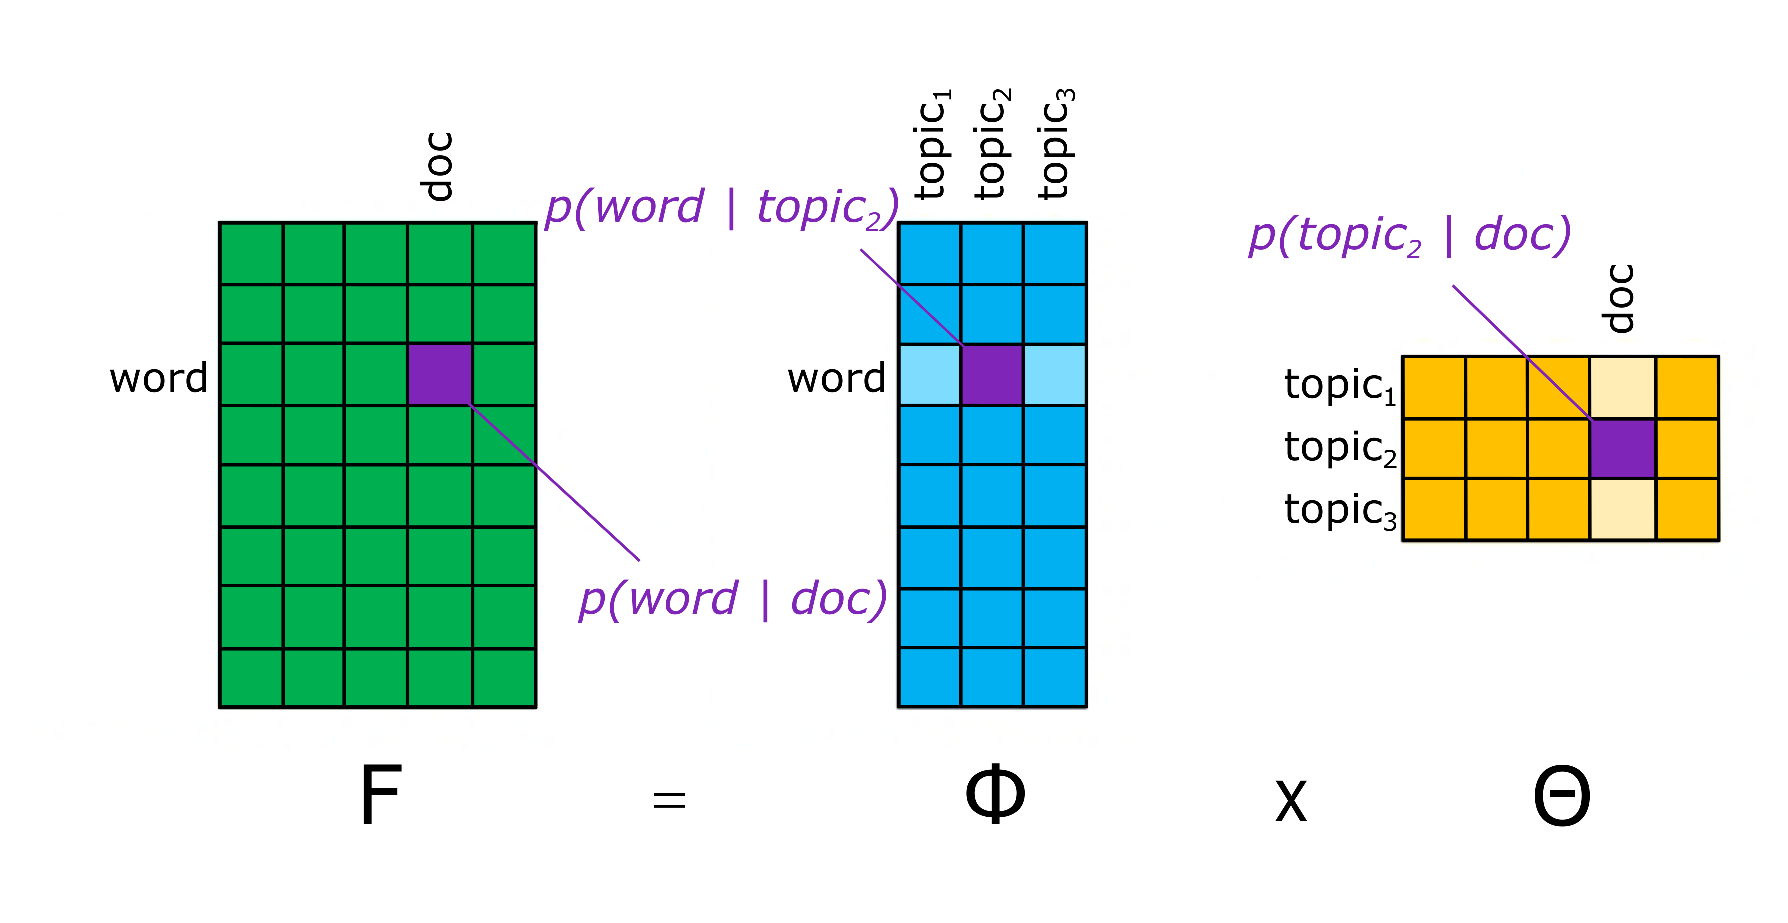
\includegraphics[width=\textwidth]{plsa_matrices.eps}
  %\end{figure}
  
  \begin{block}{Решение}
    Максимизация регуляризованного логарифма правдоподобия\footnote[frame]{Vorontsov K. et al. Bigartm: Open source library for regularized multimodal topic modeling of large collections, 2015}
    \[
      \sum_{d \in D}\sum_{w \in W_d}n_{dw} \ln{\sum_{t \in T} \phi_{wt} \theta_{td}} + R(\Phi, \Theta) \to \max\limits_{\Phi, \Theta}
    \]
  \end{block}
\end{frame}


\begin{frame}{Темы, затрагиваемые в коллекции документов}
  \begin{exampleblock}{Гипотеза о сегментной структуре текста}
    Тексты естественного языка сегментированы, состоят из сегментов разных тем.
  \end{exampleblock}
  
  \begin{block}{Следствие гипотезы}
    Слова каждой темы расположены группами, а не разбросаны по тексту беспорядочно.
  \end{block}
  
  \begin{block}{Плохие темы}
    Тема $t \in T$, найденная тематической моделью, может характеризоваться словами, которые
    \begin{itemize}
    \item вместе ни с чем не ассоциируются у человека 
    \item разбросаны по тексту в случайном порядке
    \end{itemize}
  \end{block}
\end{frame}


\begin{frame}{Качество темы $t \in T$}
  \emph{Качество темы}~---~абстрактное понятие, отражающее то, насколько хорошо распределение темы в тексте соответствует гипотезе о сегментной структуре текста.
  
  \bigskip
  
  \begin{block}{Функция качества темы $q(t)$}
    $q(t_1) < q(t_2) \leftrightarrow$ тема $t_1$ менее качественная, чем тема $t_2$
  \end{block}
  
  \begin{alertblock}{Проблема}
    $q(t)$ не известна
  \end{alertblock}
\end{frame}


\begin{frame}{Интерпретируемость темы}
  \emph{Топ\=/слова} темы~---~её самые частые слова.
  
  \medskip
  
  \emph{Интерпретируемость} означает, может ли человек по словам темы дать ей подходящее название.
  
  \vspace{0.25cm}
  
  \begin{exampleblock}{Хорошо интерпретируемая тема (самые частые слова)}
    актёр, пьеса, музыкальный, премьера, партер, зритель, продюсер, аудитория, занавес, оркестр
  \end{exampleblock}
  
  \begin{alertblock}{Плохо интерпретируемая тема (самые частые слова)}
    экспресс, эпиграф, туманный, результат, образ, право, 
    заём, иероглиф, лак, футбол
  \end{alertblock}
  
  \begin{block}{Недостаток}
    Для оценки интерпретируемости темы необходимо привлекать экспертов.
  \end{block}
\end{frame}


\begin{frame}{Когерентность по топ-словам $\coh \bigl(D, W, \phi_{\cdot t}\bigr)$}
  \begin{block}{Когерентность}
    Оценка неслучайности того, что топ\=/слова темы встречаются недалеко друг от друга в тексте.
    \[
      % \coh\Bigm|_{t}\,
      \coh \bigl(D, W, \bds{\phi}_{\cdot t}\bigr)
      = \Average\limits_{
        w_i, w_j\ \mbox{\scriptsize from } \textcolor{my-col1}{\bds k}\ \mbox{\scriptsize top-words}
      }\PMI(w_i, w_j)
    \]
  \end{block}
   
  \begin{block}{Когерентность тематической модели}
    Среднее значение когерентности по темам $T$ модели.
  \end{block}
  
  \begin{alertblock}{Недостаток}
    Частые совстречаемости \emph{определённого числа} слов темы есть лишь \emph{косвенный признак} того, что тема представлена в тексте в виде однородных сегментов.
  \end{alertblock}
\end{frame}


\begin{frame}{Когерентности по топ-словам: Ньюман, Мимно}
  \begin{block}{}
    \begin{itemize}
      \setlength\itemsep{0.5cm}
      \item
        $
        \Newman\footnote[frame]{Newman et al. Automatic Evaluation of Topic Coherence, 2010}\colon \quad \PMI(w_i, w_j) = \ln \dfrac{p(w_i, w_j)}{p(w_i) p(w_j)}
        $
      \item
        $
        \Mimno\footnote[frame]{Mimno et al. Optimizing Semantic Coherence in Topic Models, 2011}\hphantom{n\;}\colon \quad \PMI(w_i, w_j) = \ln \dfrac{D(w_i, w_j) + 1}{D(w_i)}
        $
    \end{itemize}
  \end{block}
  
  \begin{itemize}
  %\item $\textcolor{my-col1}{\bds k}$~---~number of topic $t$ top-words used to evaluate coherence
  \item $p(w_i),\, p(w_i, w_j)$~---~вероятность встретить слово $w_i$ и два слова $w_i, w_j$ в одном окне заданного размера в тексте
  \item $D(w_i),\, D(w_i, w_j)$~---~количество документов, содержащих слово $w_i$ и два слова $w_i, w_j$ в одном окне
  \end{itemize}
  
  \begin{block}{}
    \emph{Совстречаемость} слов $U \subseteq W$~---~факт нахождения двух слов $w_i, w_j \in U$ в одном текстовом окне в $W_d$ для некоторого $d \in D$.
  \end{block}
\end{frame}


\begin{frame}{Проблема когерентностей по топ-словам}
  \begin{minipage}{0.68\textwidth}
    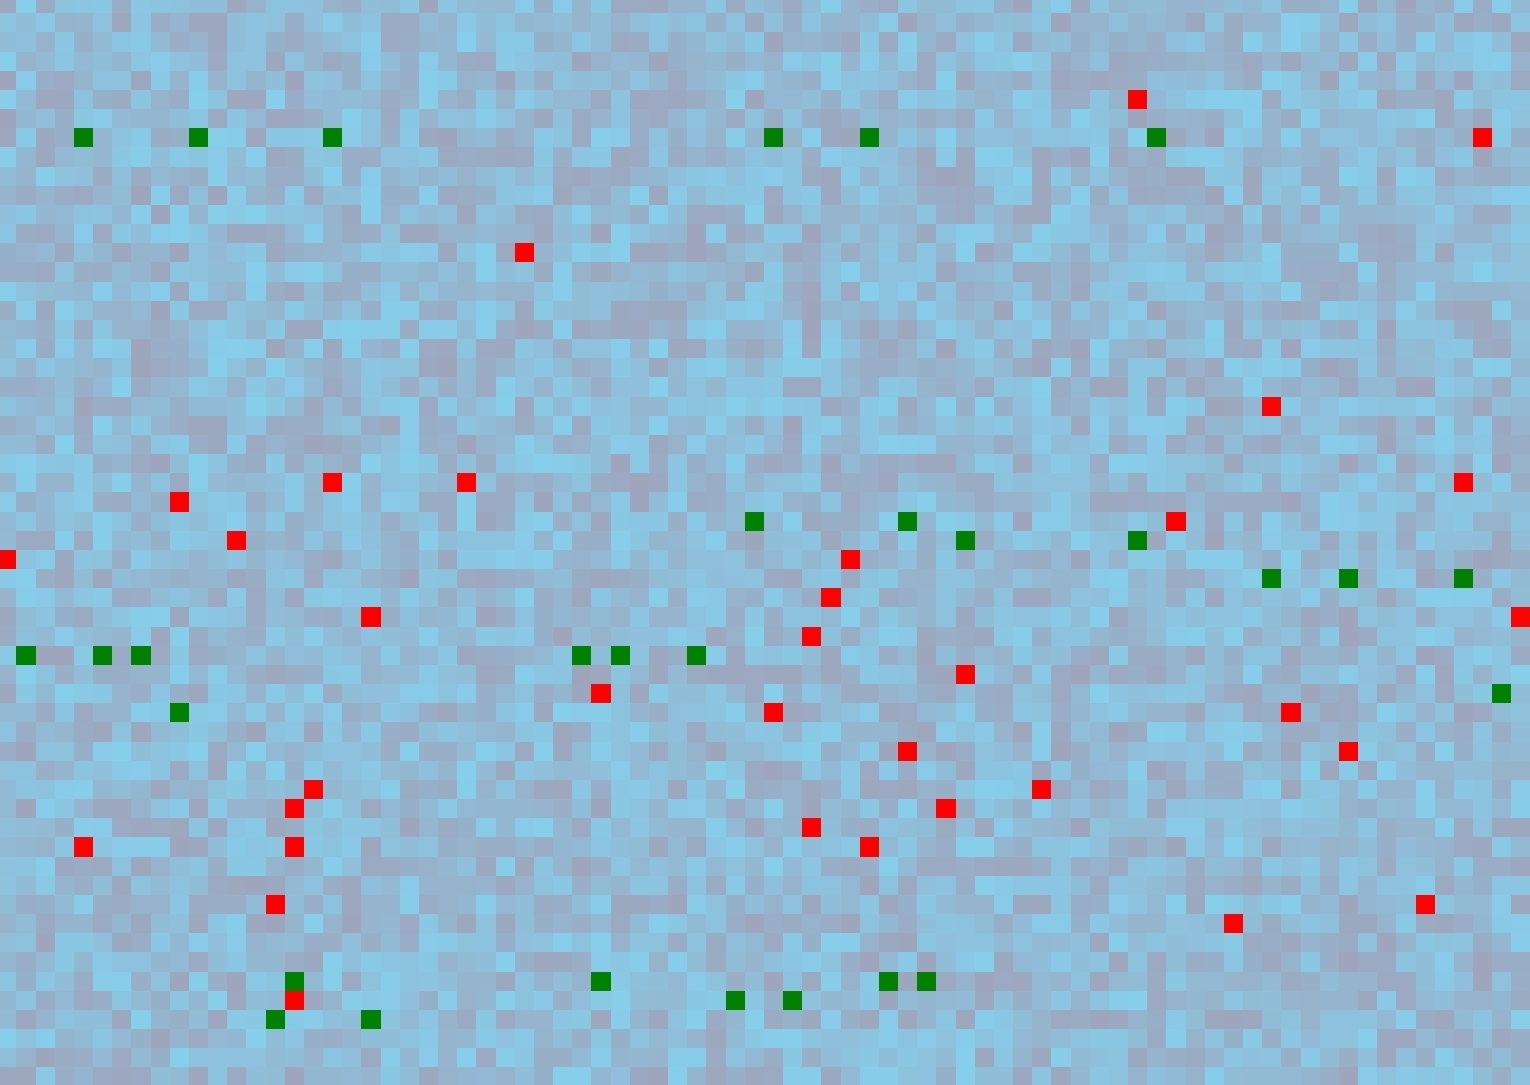
\includegraphics[width=\textwidth]{doc11358_topic0.jpg}
  \end{minipage}
  ~
  \begin{minipage}{0.28\textwidth}
    \begin{figure}[t]
      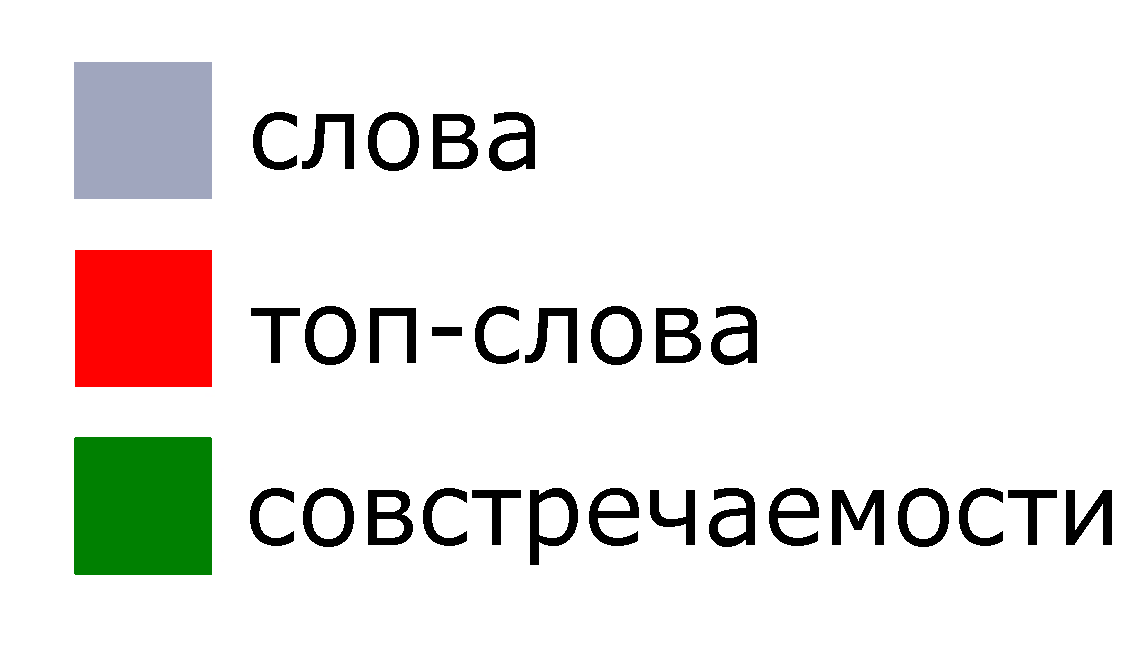
\includegraphics[width=\textwidth]{legend.eps}
    \end{figure}
  \end{minipage}

  \begin{block}{}
    Совстречаемости десяти топовых слов тем датасета из статей <<ПостНауки>>
    занимают лишь ${\bds{1.2\%}}$ от всего текста
    $\bigcup\nolimits_{d \in D} W_d$.
  \end{block}
\end{frame}


%\begin{frame}{Недостаток подхода с помощью топ\=/слов}
%  \begin{table}[h]
%    \centering
%    \captionsetup{justification=centering}
%    
%    \begin{tabular}{lcc}
%      % {} & ПостНаука, \%\\% & Википедия, \%\\
%      \toprule
%      Min & $0.016$\\% & 0.0065\\
%      Median & $0.048$\\% & 0.029\\
%      Mean & $0.062$\\% & 0.036\\
%      Max & $0.28$\\% & 0.11\\
%      \midrule
%      Total & $\mathbf{1.2}$\\% & \textbf{1.7}
%      \bottomrule
%    \end{tabular}
%    \vspace{0.5cm}
%    \caption*{Часть корпуса (\%), которая занята совстречаемостями десяти топовых слов для тем <<ПостНауки>>}
%  \end{table}
%\end{frame}


\begin{frame}{Проблема когерентностей по топ-словам}
  \begin{block}{}
    Во фрагменте текста есть \emph{только одно} слово <<частиц>> из списка 10 топ\=/слов темы <<физика>>, и \emph{ни одной} совстречаемости.
    %Широкий спектр других слов темы будет проигнорирован когерентностями по топ\=/словам. 
  \end{block}
  
  \begin{figure}[h]
    \centering
    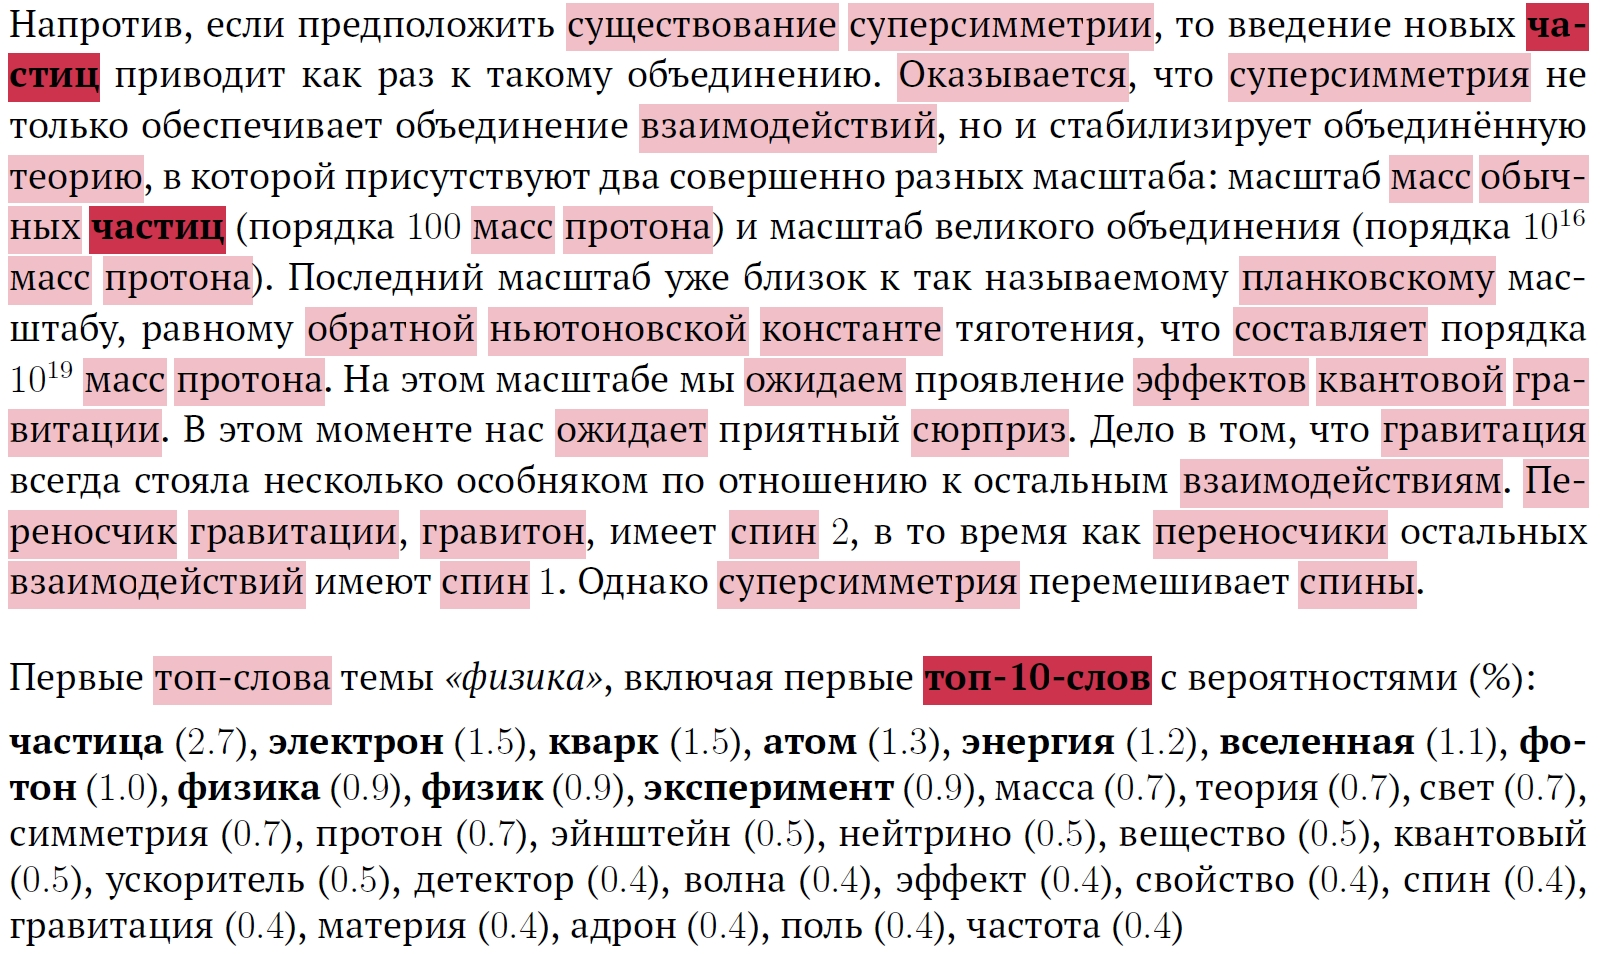
\includegraphics[width=1.0\textwidth]{topwords-insufficient.jpg}
  \end{figure}
\end{frame}


%\section{Цель исследования}
\begin{frame}{Цель исследования}
  \begin{block}{Проблема}
    Когерентности по топ\=/словам учитывают не всю информацию о тематической модели
    % Помимо этого, оценивать интерпретируемость с помощью экспертов дорого и затратно.
  \end{block}
  \begin{block}{Решение}
    Смотреть распределение темы по \emph{всем} словам текста
    %Считать когерентность темы как среднюю схожесть слов, близко расположенных в тексте.
  \end{block}
  \begin{block}{Задачи}
    \begin{itemize}
      \item Предложить новые методы подсчёта когерентности
      \item Сравнить с существующими, основанными на совстречаемостях топ\=/слов
    \end{itemize}
  \end{block}
\end{frame}


%\begin{frame}
%  \frametitle{Содержание}
%  \tableofcontents
%\end{frame}


\begin{frame}{Внутритекстовая когерентность $\coh \bigl(D, W, \Phi, \Theta\bigr)$}
  \begin{block}{Semantic Closeness (SemantiC)}
    % Близость векторов близко расположенных в тексте слов темы $t$
    \begin{flalign*}
      &\SemantiC_{l_2}\Bigm|_{\textcolor{my-col1}{t}} = \biggl\langle\bigl[0 < j \hm- i < \window\bigr]\; {-}\bigl\|\bsym{w_i} - \bsym{w_j}\bigr\|_2\biggr\rangle_{\substack{w_i,\, w_j \in \bigcup_d W_d\\\argmax_s \bds{w}_i(s) = \textcolor{my-col1}{t}\\\argmax_s \bds{w}_j(s) = \textcolor{my-col1}{t}}}&
    \end{flalign*}
    
    % Разброс темы $t$ по близко расположенным словам
    \begin{flalign*}
      &\SemantiC_{\Var} \Bigm|_{\textcolor{my-col1}{t}} = \biggl\langle{-}\Var\Bigl(\bsym{w}_i(\textcolor{my-col1}{t}), \bsym{w}_{i+1}(\textcolor{my-col1}{t}), \ldots, \bsym{w}_{i+\window}(\textcolor{my-col1}{t})\Bigr)\biggr\rangle_{w_i\in \bigcup_d W_d}&
    \end{flalign*}
  \end{block}
  
  \begin{flalign*}
    &W_d \ni w \mapsto \bds{w} \equiv \bigl(p(t \mid d, w)\bigr)_{t \in T}&
  \end{flalign*}
\end{frame}


\begin{frame}{Внутритекстовая когерентность $\coh \bigl(D, W, \Phi, \Theta\bigr)$}
  \begin{block}{Topic Length (TopLen)}
    % Средняя длина темы $t$ внутри текста
    \begin{flalign*}
      &\TopLen \Bigm|_{\textcolor{my-col1}{t}} =
        \biggl\langle \overbrace{l(0)}^{l_1}, \overbrace{l(l_1)}^{l_2}, l(l_1 + l_2), \ldots, l\left(\sum_{r=0}^{k-1} l_r\right), \ldots \biggr\rangle_{l_j > 0}&
    \end{flalign*}
  \end{block}
  
  \begin{flalign*}
    &l(\cdot) : \begin{aligned}
      &\left\{\begin{aligned}
        &l(i) = \max\Bigl\{L : \threshold + \sum\limits_{j=i}^{i + L}
          \Bigl( \bsym{w}_j(\textcolor{my-col1}{t}) - \underset{\substack{1 \leq \tau \leq |T|\\\tau \not= t}}{\max}\, \bsym{w}_j(\tau) \Bigr) \geq 0\Bigr\}\\
        &\argmax\nolimits_s \bsym{w}_{i}(s) = \textcolor{my-col1}{t}
      \end{aligned}\right.\\
      &\left\{\begin{aligned}
        &l(i) = 0\\
        &\argmax\nolimits_s \bsym{w}_{i}(s) \not= \textcolor{my-col1}{t}
      \end{aligned}\right.
    \end{aligned}&
  \end{flalign*}
  
  \begin{flalign*}
    &W_d \ni w \mapsto \bds{w} \equiv \bigl(p(t \mid d, w)\bigr)_{t \in T}&
  \end{flalign*}
\end{frame}


\begin{frame}{Внутритекстовая когерентность $\coh \bigl(D, W, \Phi, \Theta\bigr)$}
  \begin{block}{Focus Consistency (FoCon)}
    % Как сильно изменяется тема $t$ среди смежных слов
    \begin{flalign*}
      &\FoCon =
        {-}\sum\limits_{d \in D}\sum\limits_{\substack{w_i, w_j \in W_d\\j-i=1}}
        \bigl|\bsym{w}_i(t) - \bsym{w}_j(t)\bigr| +
        \bigl|\bsym{w}_i(\tau) - \bsym{w}_j(\tau)\bigr|&\\
      &\left\{\begin{aligned}
          &t = \argmax\nolimits_s \bds{w}_i(s)\\
          &\tau = \argmax\nolimits_s \bds{w}_j(s)
        \end{aligned}\right.&
    \end{flalign*}   
  \end{block}
  
  \begin{flalign*}
    &W_d \ni w \mapsto \bds{w} \equiv \bigl(p(t \mid d, w)\bigr)_{t \in T}&
  \end{flalign*}
  
  \begin{block}{}
    Метод не привязан к теме, а даёт значение когерентности для \emph{тематической модели} как целого.
  \end{block}
\end{frame}


\begin{frame}{Качество функций когерентности}
  \begin{exampleblock}{Гипотеза о сегментной структуре текста}
    Тексты естественного языка сегментированы, состоят из сегментов разных тем.
  \end{exampleblock}
  
  \begin{block}{Следствие}
    Чем лучше функция когерентности, тем лучше она должна описывать способность тематической модели угадывать сегментную структуру текста.
  \end{block}
  
  \begin{block}{Проблема}
    Позиции сегментов не известны.
  \end{block}
  
  \begin{block}{Решение: полусинтетический датасет}
    $2000$ \emph{монотематических} статей <<ПостНауки>> разрезаются на сегменты одинаковой длины, которые потом сшиваются в новые документы $D'$.
  \end{block}
  %\footnote[frame]{https://postnauka.ru}
\end{frame}


\begin{frame}{Методы оценки качества сегментации текста}
  \begin{block}{Segmentation quality (sq)}
    \begin{flalign*}
      &sq(D', W, \Phi', \Theta') \Bigm|_{\textcolor{my-col1}{t'}} =
        \sum\limits_{d \in D'} \sum\limits_{\substack{w' \in W'_{d'}\\\argmax_s \bds{w}(s) = \textcolor{my-col1}{t}}}
          p(t' \mid d', w')&
    \end{flalign*}
  \end{block}
  
  \vspace{-0.25cm}
  
  \begin{flalign*}
    &\left\{\begin{aligned}
      &W_d \ni w \mapsto w' \in W'_{d'}\\
      &W_d \ni w \mapsto \bds{w} \equiv \bigl(p(t \mid d, w)\bigr)_{t \in T}\\
      &T \ni \textcolor{my-col1}{t} \leftrightarrow \textcolor{my-col1}{t'} \in T'
    \end{aligned}\right.&
  \end{flalign*}
  
  \begin{block}{Гипотеза}
    Функция $sq(\cdot)$ задаёт тот же порядок на образах тем $T'$, что и неизвестная функция качества тем $q(\cdot)$ на исходных темах $T$
    \[sq(t_1') < sq(t_2') \leftrightarrow q(t_1) < q(t_2)\]
  \end{block}
\end{frame}


\begin{frame}{Корреляция между когерентностями и качеством сегментации}
  \begin{block}{Ряд моделей}
    \[\Phi'(\alpha) = \alpha \cdot \Phi_{bad} + (1 - \alpha) \cdot \Phi_{good}\ \bigm|\ \alpha \in [0, 1)\]
    \noi
    $\Phi_{good}$~---~модель исходной коллекции <<ПостНауки>>\sp
    $\Phi_{bad}$~---~случайная из $\Dirichlet\bigl(0.01^{|W|}\bigr)$
  \end{block}
  
  \begin{block}{Корреляция (по Спирмену)}
    \[\Corr\Bigl\{ \bigl(\coh(\Phi'(\alpha))\bigr)_\alpha,
      \bigl(sq(\Phi'(\alpha))\bigr)_\alpha \Bigr\}\]
  \end{block}
\end{frame}


\begin{frame}{Результаты корреляций}
  \begin{table}[t]
    %\begin{subtable}{0.32\textwidth}
    %  \begin{tabular}{lr}
    %    Coh & Corr\\
    %    \midrule
    %    $\Newman$ & $0.75$\\
    %    $\Mimno$ & $0.96$\\
    %    % \midrule
    %    $\SC_{l_2}$ & $0.92$\\
    %    % $\SC {\Cos}$ & $-0.97$\\
    %    $\SC_{\Var}$ & $\mathbf{1.00}$\\
    %    $\TopLen$ & $\mathbf{1.00}$\\
    %    $\FoCon$ & $\mathbf{1.00}$\\
    %    % \bottomrule
    %  \end{tabular}
    %\end{subtable}
    %~
    %\begin{subtable}{\textwidth}
      \begin{tabular}{lr}
        Coh & Corr\\
        \midrule
        $\Newman$ & $0.80$\\
        $\Mimno$ & $0.94$\\
        % \midrule
        $\SemantiC_{l_2}$ & $0.70$\\
        % $\SemantiC {\Cos}$ & $-0.97$\\
        $\SemantiC_{\Var}$ & $\mathbf{1.00}$\\
        $\TopLen$ & $\mathbf{1.00}$\\
        $\FoCon$ & $\mathbf{1.00}$\\
        % \bottomrule
      \end{tabular}
    %\end{subtable}
    %~
    %\begin{subtable}{0.32\textwidth}
    %  \begin{tabular}{lr}
    %    Coh & Corr\\
    %    \midrule
    %    $\Newman$ & $0.85$\\
    %    $\Mimno$ & $0.97$\\
    %    % \midrule
    %    $\SC_{l_2}$ & $0.59$\\
    %    % $\SC {\Cos}$ & $-0.96$\\
    %    $\SC_{\Var}$ & $\mathbf{1.00}$\\
    %    $\TopLen$ & $\mathbf{1.00}$\\
    %    $\FoCon$ & $\mathbf{1.00}$\\
    %    % \bottomrule
    %  \end{tabular}
    %\end{subtable}
    \centering
    \captionsetup{justification=centering}
    \caption*{
      Корреляции при размере сегментов $200$ %$50$, $200$ и $400$
      слов\\и при $5$ темах в каждом сшитом из сегментов документе
    }
  \end{table}
\end{frame}


\begin{frame}{Когерентности (синие) и качество сегментации (красное) как функции качества тематической модели}
  % dataset $\sgm=200,\ \thm=5$
  
  \begin{figure}[h]
    \begin{subfigure}[t]{0.48\textwidth}
      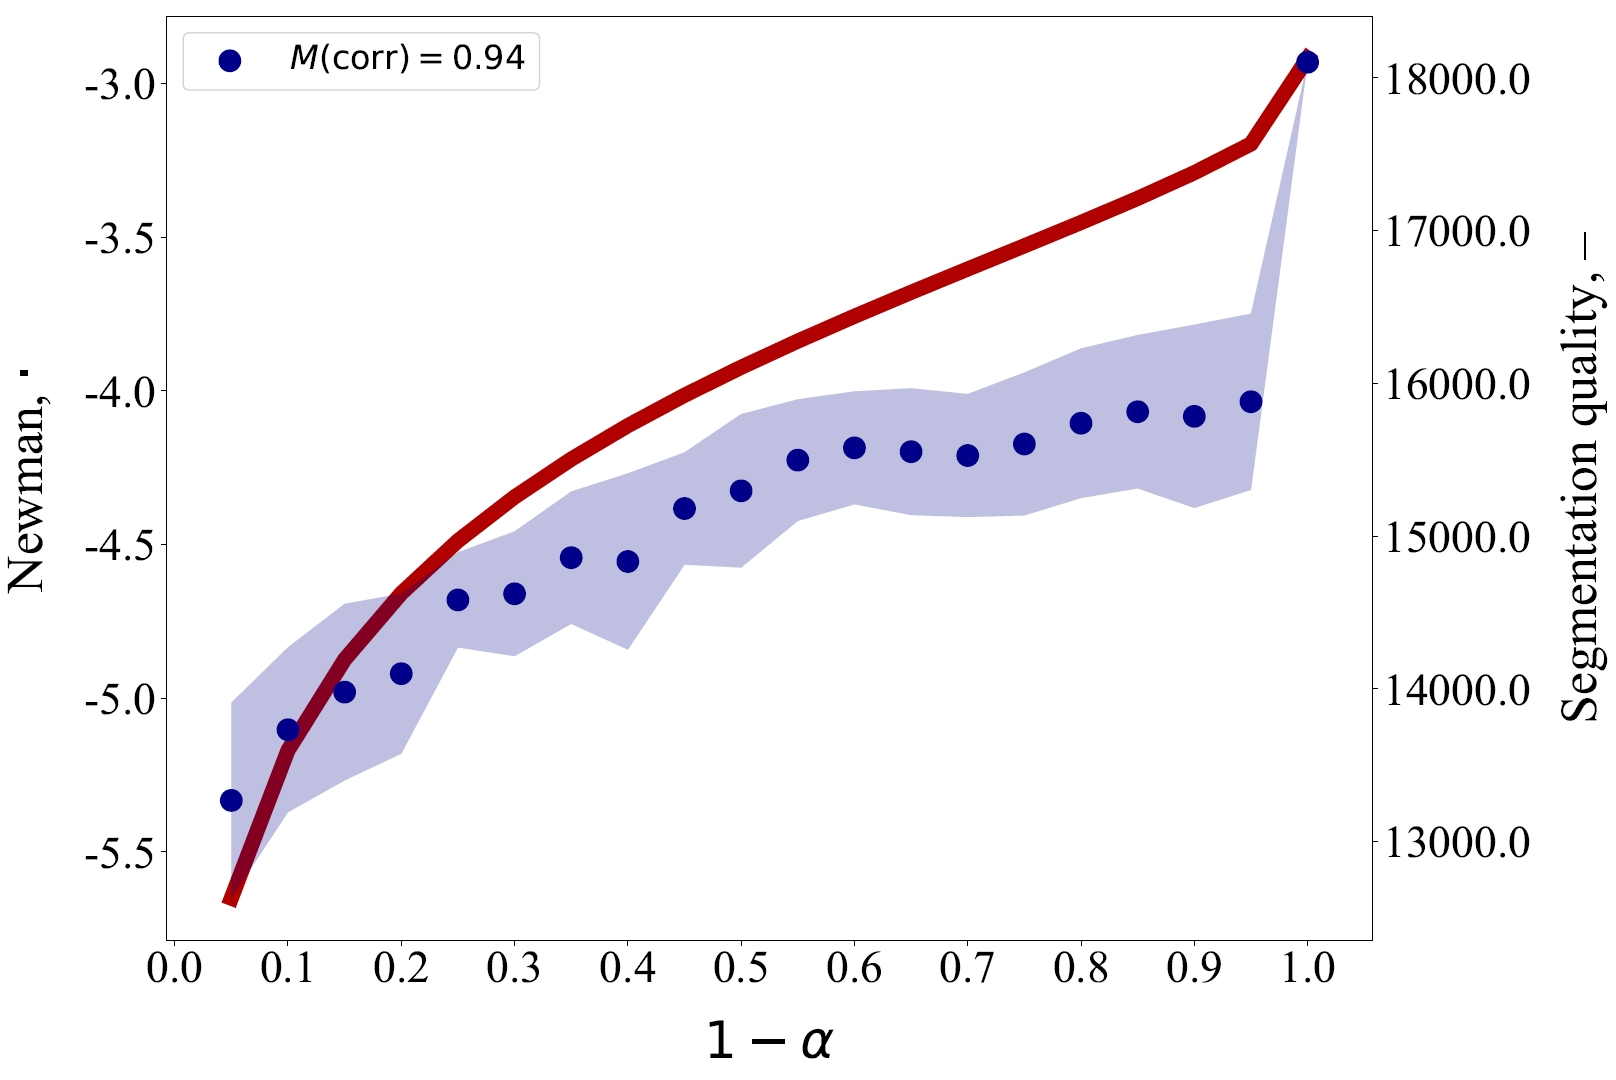
\includegraphics[width=\linewidth]{newman-iteration.jpg}
    \end{subfigure}
    ~
    \begin{subfigure}[t]{0.48\textwidth}
      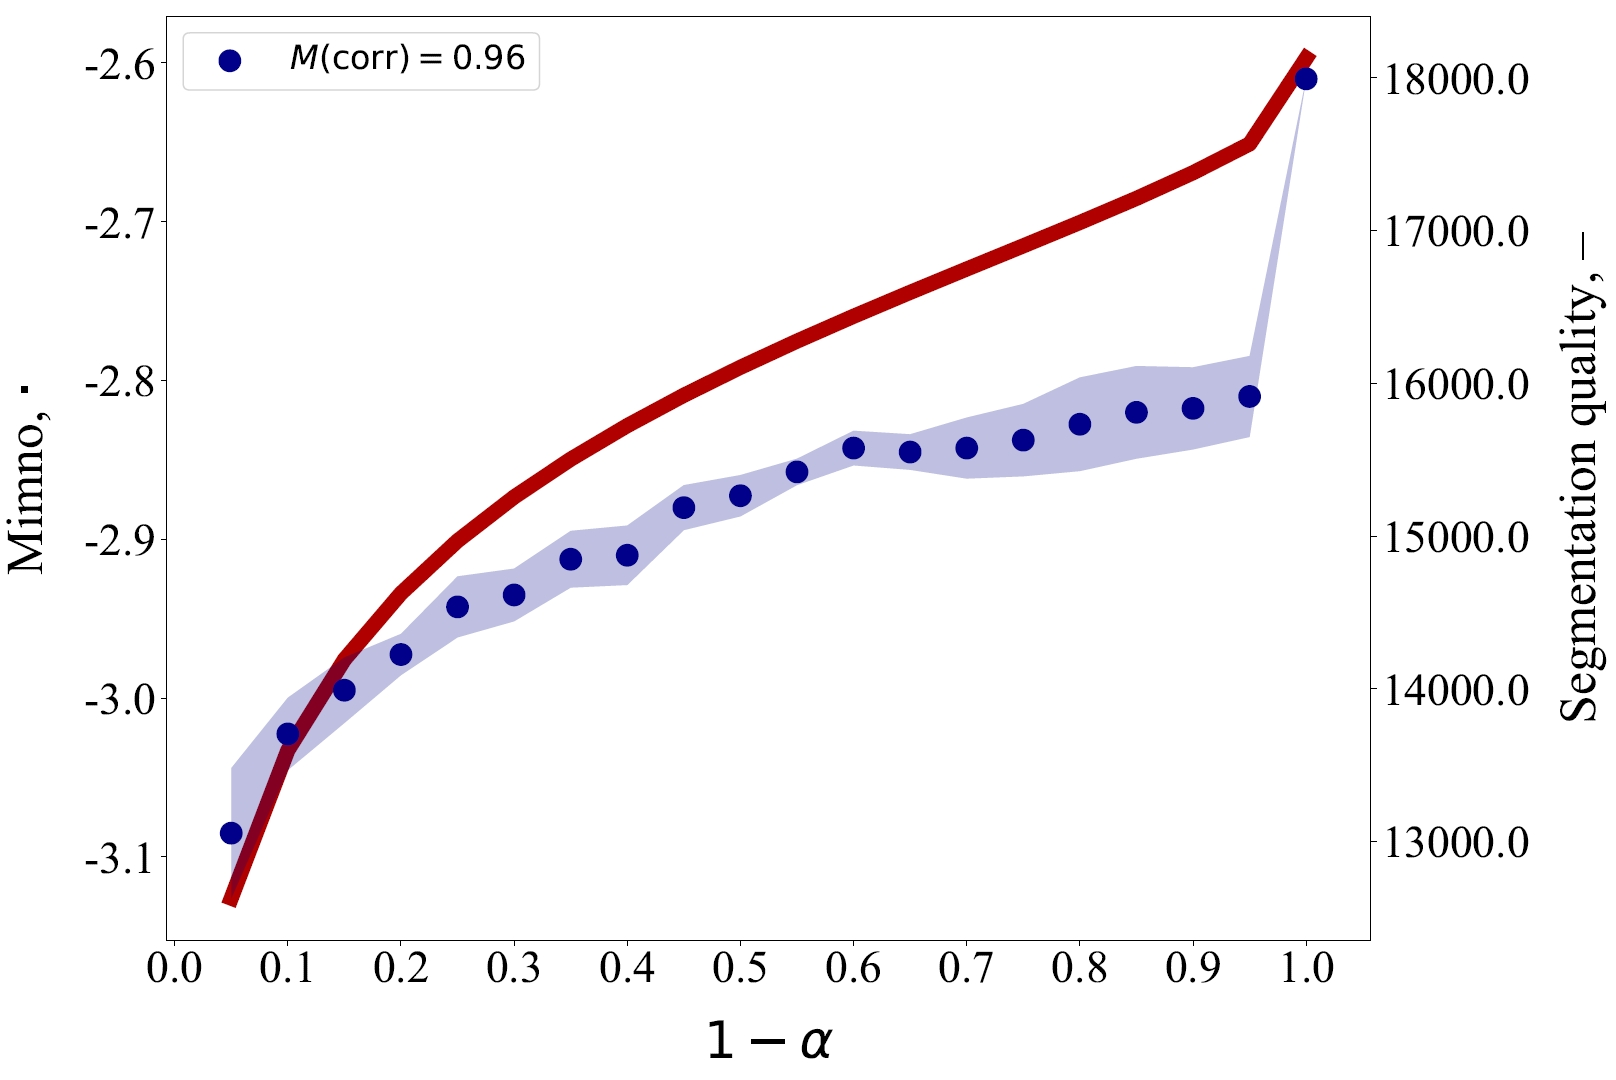
\includegraphics[width=\linewidth]{mimno-iteration.jpg}
    \end{subfigure}
    %%
    \begin{subfigure}[t]{0.48\textwidth}
      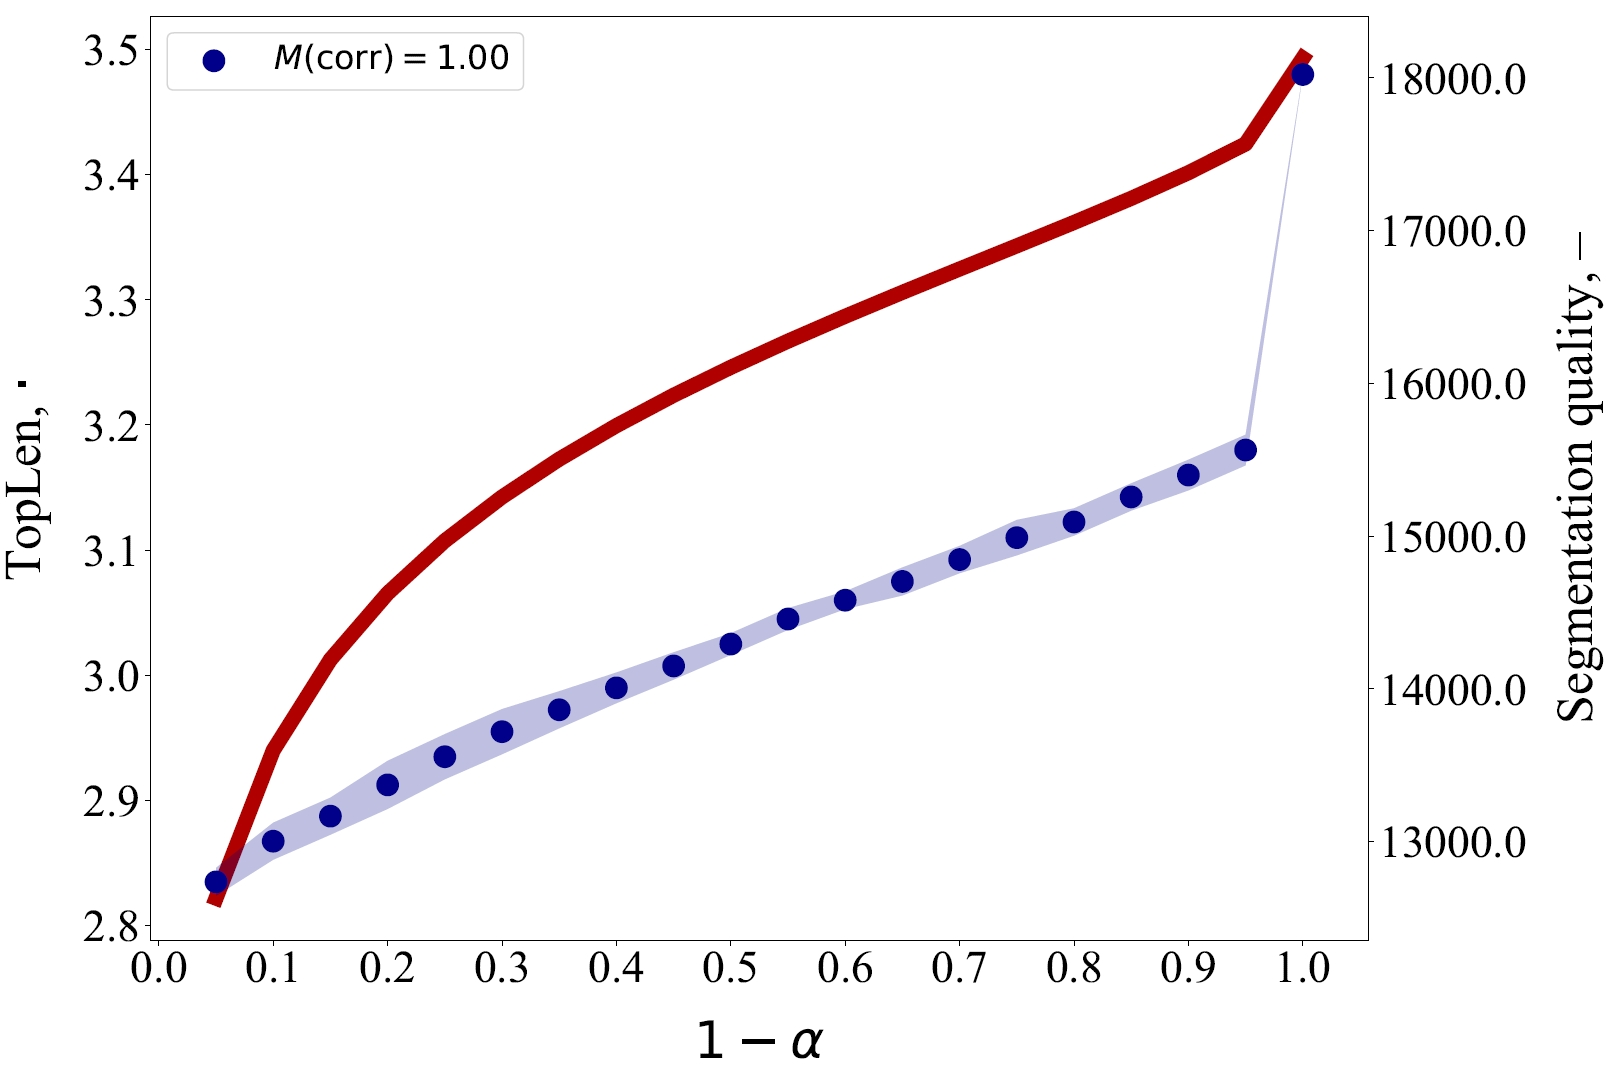
\includegraphics[width=\linewidth]{toplen-iteration.jpg}
    \end{subfigure}
    ~
    \begin{subfigure}[t]{0.48\textwidth}
      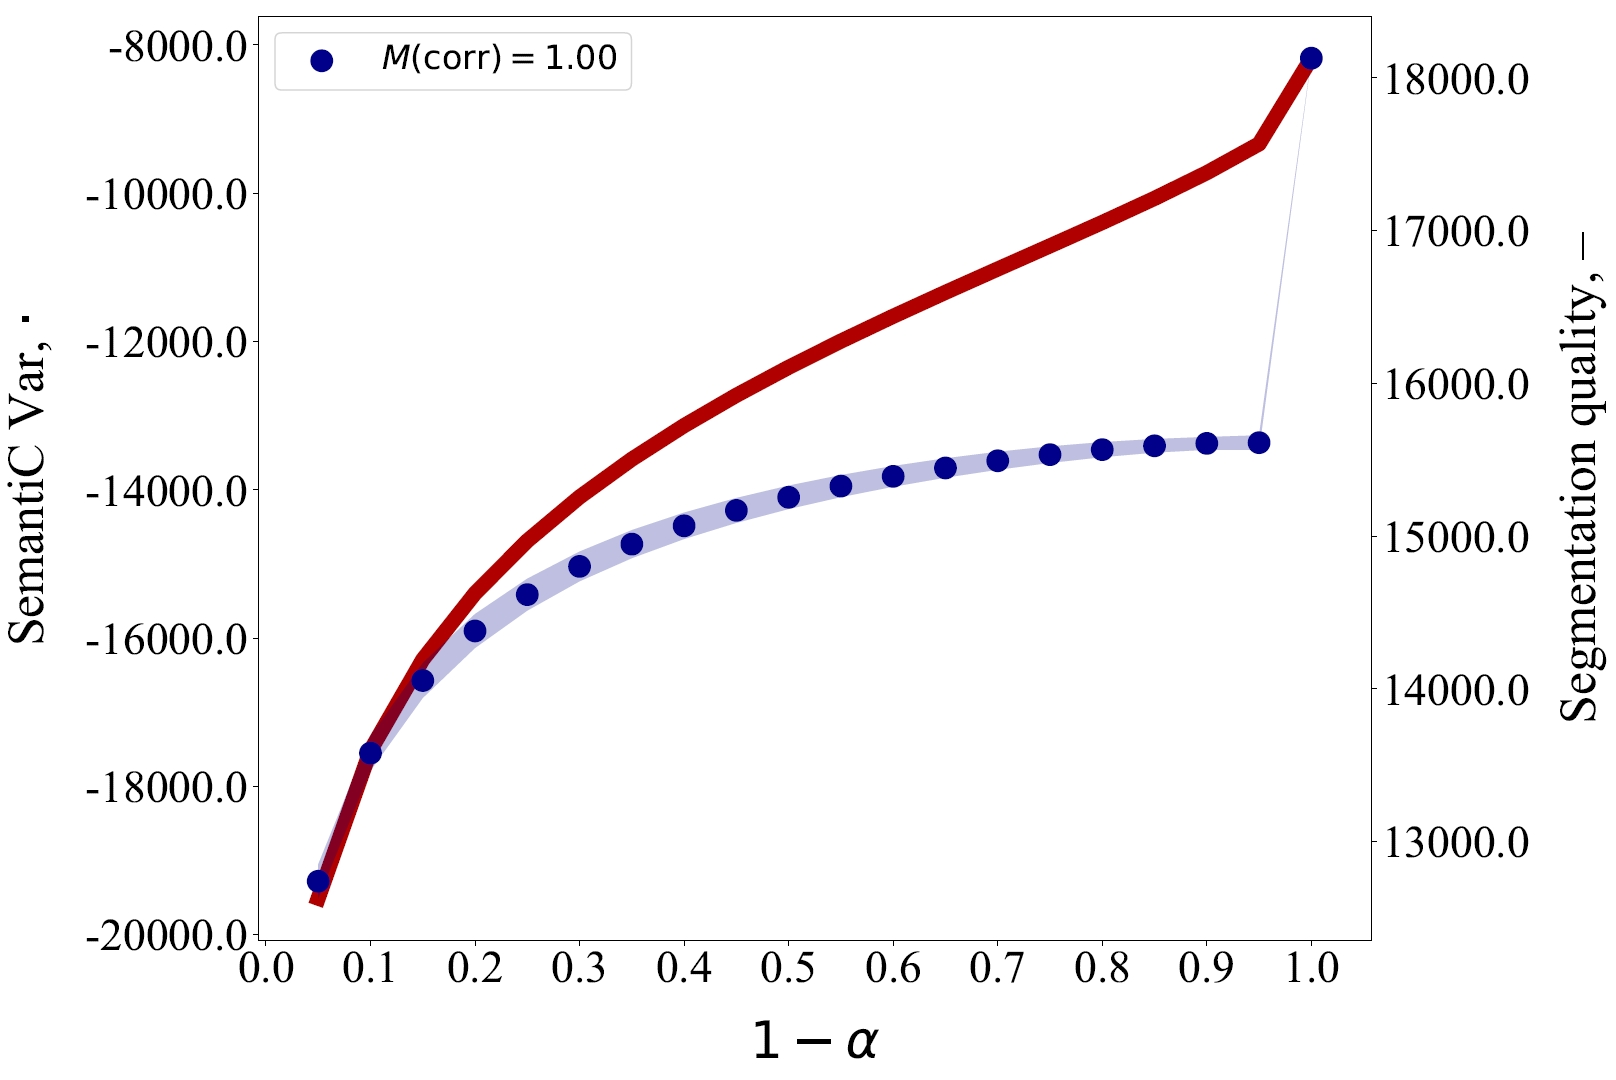
\includegraphics[width=\linewidth]{semantic_var-iteration.jpg}
    \end{subfigure}
  \end{figure}
\end{frame}


\begin{frame}{Результаты}
  \begin{itemize}%\setlength\itemsep{0.5cm}
  \item Проиллюстрирован недостаток когерентностей по топ-словам: покрытие лишь малой части текстовой коллекции.

  \item Предложен полуавтоматический метод оценки качества функций когерентности: по корреляции с качеством сегментации полусинтетического текста тематическими моделями.

  \item Представлены методы \emph{внутритекстовой} когерентности.
    По предложенной функции качества некоторые внутритекстовые методы лучше, чем когерентности по топ\=/словам.
  \end{itemize}
  
  \begin{block}{Публикация}
    Alekseev V. A., Bulatov V. G., Vorontsov K. V.\\Intra-Text Coherence as a Measure of Topic Models' Interpretability // Computational Linguistics and Intellectual Technologies. Dialogue 2018. Pp. 1-13.
  \end{block}
\end{frame}
\end{document}